\chapter{Energía, curvatura y radiación}

\lectureoverview{El modelo newtoniano resulta mucho más revelador cuando se eliminan dos restricciones. En primer lugar, una galaxia comóvil no tiene por qué tener una energía total exactamente nula; dejar su energía sin fijar introduce el término \(a^{-2}\), que la relatividad general reinterpretará como curvatura espacial. En segundo lugar, la fuente cósmica no tiene por qué ser materia sin presión. Las longitudes de onda de los fotones se estiran con el factor de escala, de modo que la radiación se diluye como \(a^{-4}\) y da lugar a la ley \(a(t)\propto t^{1/2}\). Por tanto, un universo que contiene tanto materia como radiación está dominado por la radiación para valores pequeños de \(a\) y por la materia para valores mayores de \(a\). En el proceso distinguiremos el movimiento newtoniano local de la geometría relativista global e identificaremos las preguntas que no pueden resolverse sin la relatividad general.}

\section{Lo que puede explicar Newton}

Antes de ampliar el modelo, conviene preguntarse por qué funcionó el cálculo newtoniano anterior. El universo físico se describe mediante la relatividad general, y su geometría espacial no tiene por qué ser euclídea en términos globales. Sin embargo, todo espacio curvo y suave es aproximadamente plano en un entorno suficientemente pequeño. Una pequeña zona de la superficie terrestre parece plana; del mismo modo, una región del universo mucho menor que su radio de curvatura puede tratarse como plana.

``Pequeña'' es una noción relativa a la escala de curvatura. La región aún puede extenderse miles de millones de años luz. En ella, las galaxias vecinas pueden describirse con la mecánica newtoniana si sus velocidades peculiares relativas son no relativistas y el campo gravitatorio es débil. Por tanto, el cálculo newtoniano no compite con la teoría de Einstein: es el límite local de movimientos lentos de una descripción más completa.

Hay una advertencia inmediata: la radiación no se mueve lentamente. Los fotones, y también los neutrinos mientras sean relativistas, no pueden tratarse como un gas de partículas newtonianas ordinarias. El razonamiento newtoniano seguirá organizando la ecuación de expansión, pero habrá que ampliar la fuente que aparece en su lado derecho: de densidad de masa en reposo a densidad de energía. Aquí es donde la aproximación empieza a revelar sus propios límites.

\section{Recordatorio sobre el factor de escala}

Consideremos una distribución homogénea de galaxias y asociemos coordenadas a una cuadrícula que se mueve con el flujo cósmico medio. Una galaxia situada en la coordenada comóvil fija \(x\) tiene una distancia física
\begin{equation}
D(t)=a(t)x
\label{eq:c02-distance}
\end{equation}
respecto del origen elegido. El factor de escala \(a(t)\) convierte la separación entre coordenadas en separación física.

El valor absoluto de \(a\) es convencional. Si se reescalan todas las coordenadas comóviles mediante una constante, las mismas distancias físicas pueden representarse con el reescalamiento inverso de \(a\). Así, ni \(a\) ni la masa asignada a una celda de coordenadas son invariantes por separado. En cambio, sí son invariantes los cocientes entre factores de escala y la tasa de expansión fraccional:
\begin{equation}
\frac{a(t_2)}{a(t_1)},
\qquad
H(t)\equiv\frac{\dot a}{a}.
\label{eq:c02-hubble}
\end{equation}
En efecto, si \(a'=\alpha a\) para una constante fija \(\alpha\), entonces \(\dot a'/a'=\dot a/a\).

Sea \(\nu_m\) la masa contenida en una unidad de volumen de coordenadas comóviles. Su valor numérico cambia si se cambia la etiqueta de la cuadrícula, pero permanece constante en el tiempo si se conserva la materia ordinaria. Un cubo comóvil unitario tiene un volumen físico de \(a^3\), por lo que la densidad de materia es
\begin{equation}
\boxed{\rho_m(a)=\frac{\nu_m}{a^3}.}
\label{eq:c02-matter-density}
\end{equation}
Esta dilución como \(a^{-3}\) se debe simplemente al aumento del volumen: la energía en reposo dentro de la caja comóvil permanece fija mientras su volumen crece.

Las galaxias reales no están fijadas rígidamente a la cuadrícula. Orbitan en grupos, caen en cúmulos y tienen pequeñas velocidades respecto del flujo medio. El factor de escala describe el movimiento suavizado a gran escala; esas desviaciones locales se llaman \emph{velocidades peculiares}.

\begin{classroomqa}
\audiencequestion{¿Tiene que moverse cada galaxia exactamente en dirección radial, alejándose de todas las demás?}
\lecturerresponse{Solo el flujo de Hubble promediado tiene esa forma. El movimiento real de una galaxia es la suma de la expansión común y una velocidad peculiar causada por las estructuras cercanas. La distinción es como la que hay entre la corriente de un río y los remolinos superpuestos a ella: estos influyen localmente sin borrar el flujo a gran escala. \lecturetimestamp{00:24:47--00:26:33}}
\end{classroomqa}

Para materia sin presión y con energía total newtoniana nula, la clase anterior obtuvo
\begin{equation}
H^2=\frac{8\pi G}{3}\rho_m
=\frac{8\pi G\nu_m}{3a^3}.
\label{eq:c02-zero-energy-friedmann}
\end{equation}
Como la normalización global de la cuadrícula es arbitraria, podemos elegir provisionalmente unidades tales que \(8\pi G\nu_m/3=1\). En la rama expansiva,
\begin{equation}
\frac{\dot a}{a}=\frac{1}{a^{3/2}},
\qquad
\dot a=\frac{1}{\sqrt a}.
\end{equation}
Invertir la derivada e integrar da
\begin{equation}
\frac{dt}{da}=\sqrt a,
\qquad
t-t_B=\frac{2}{3}a^{3/2},
\end{equation}
donde \(t_B\) es el instante en que esta solución idealizada alcanza \(a=0\). Por tanto,
\begin{equation}
\boxed{a(t)\propto (t-t_B)^{2/3}.}
\label{eq:c02-matter-law}
\end{equation}
El universo se expande para siempre en este modelo crítico compuesto solo por materia. Su expansión se ralentiza porque \(\dot a\propto a^{-1/2}\), pero \(\dot a\) no se anula para ningún valor finito de \(a\).

\begin{figure}[ht]
\centering
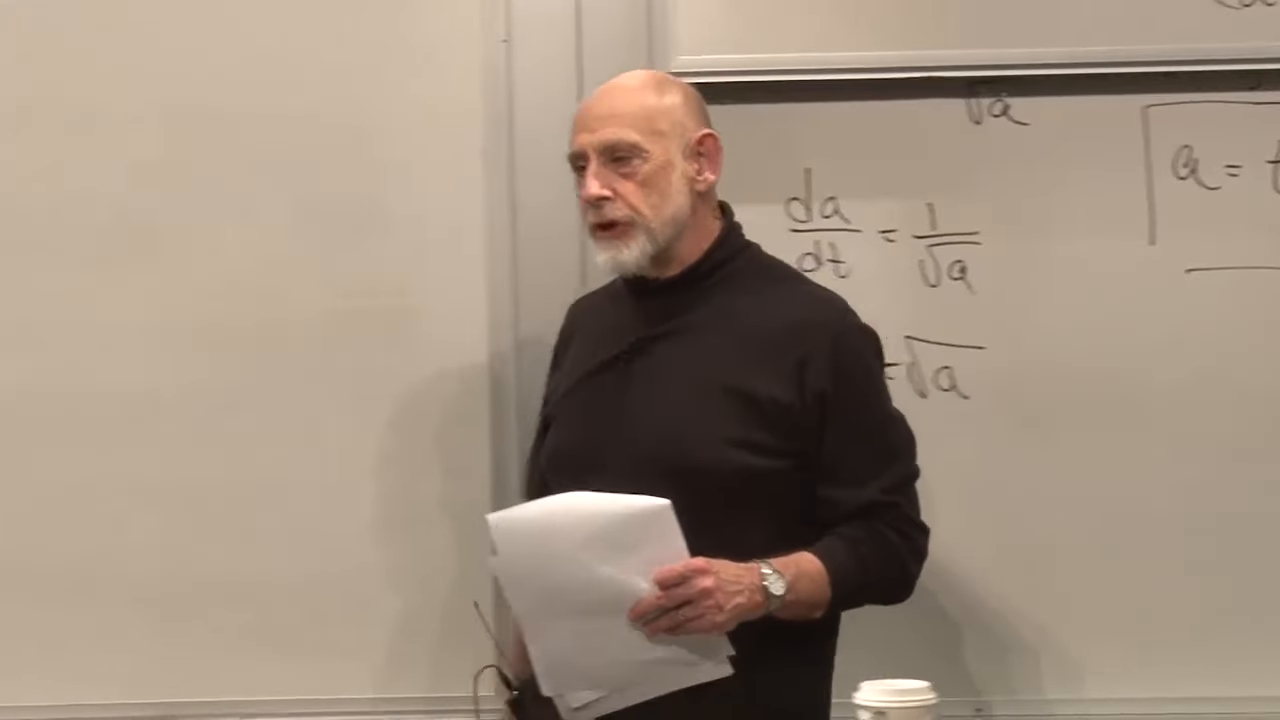
\includegraphics[width=0.68\textwidth]{lecture_02_figure_02.png}
\caption{El esquema de repaso recoge \(\dot a=1/\sqrt a\) y la ley encuadrada para el dominio de la materia \(a\propto t^{2/3}\). Parte del álgebra intermedia está oculta y se proporciona en las ecuaciones~\eqref{eq:c02-zero-energy-friedmann}--\eqref{eq:c02-matter-law}.}
\label{fig:c02-matter-recap}
\lectureframe{00:29:20.838}
\end{figure}

\begin{classroomqa}
\audiencequestion{¿Por qué se descartó la raíz cuadrada negativa?}
\lecturerresponse{La ecuación no la descarta. La ecuación~\eqref{eq:c02-zero-energy-friedmann} fija \(H^2\), pero no el signo de \(H\). La raíz positiva describe la expansión y la negativa, la contracción. Una roca en el campo gravitatorio de un planeta puede moverse hacia fuera o hacia dentro y obedecer la misma ecuación de energía; la condición inicial determina la rama. Elegimos la rama expansiva porque ese es el universo que estamos estudiando. \lecturetimestamp{00:23:09--00:24:46}}
\end{classroomqa}

El siguiente modelo seguirá omitiendo la energía oscura. La omisión es deliberada: primero entenderemos el marco anterior de materia y radiación antes de añadir el componente que controla la era actual de expansión acelerada. En cambio, la materia oscura ya está incluida en el término de materia, porque la materia oscura no relativista también se diluye como \(a^{-3}\).

\begin{classroomqa}
\audiencequestion{¿Acaso la energía oscura no es hoy el componente dominante?}
\lecturerresponse{Sí. La descripción con dos componentes que desarrollamos aquí corresponde a la cosmología pedagógica estándar anterior al descubrimiento de la aceleración actual. La materia oscura se incluye con la materia; la energía oscura es un tercer componente que se introducirá por separado. Empezar por el modelo anterior nos permite ver qué cambia con cada término adicional. \lecturetimestamp{00:28:02--00:28:45}}
\end{classroomqa}

\section{Restablecimiento de la constante de energía}

La elección de energía nula es una condición inicial especial. Para eliminarla, volvamos a una galaxia de masa \(m\) situada en el borde de una esfera homogénea. Sea \(x\) su radio comóvil, de modo que
\begin{equation}
D=ax,
\qquad
\dot D=\dot a x.
\label{eq:c02-comoving-particle}
\end{equation}
El teorema de las capas de Newton establece que solo la masa \(M(D)\) dentro de la esfera afecta a la aceleración radial; las capas esféricas exteriores no ejercen fuerza neta. La energía newtoniana conservada de la galaxia es
\begin{equation}
\frac{1}{2}m\dot D^{\,2}-\frac{GM(D)m}{D}=E.
\label{eq:c02-newton-energy}
\end{equation}
El factor \(m\) debe aparecer en ambos términos. Es fácil omitirlo al escribir deprisa en la pizarra, pero conservarlo deja claro que la constante final es la energía por unidad de masa de prueba.

La homogeneidad nos permite elegir la galaxia representativa en \(x=1\). Entonces \(D=a\), \(\dot D=\dot a\), y la esfera tiene
\begin{equation}
V_{\rm sph}=\frac{4\pi}{3}a^3,
\qquad
M(a)=\rho_m V_{\rm sph}=\frac{4\pi}{3}\rho_m a^3.
\label{eq:c02-enclosed-mass}
\end{equation}
En la pizarra se usa \(V\) tanto para el volumen como, en una anotación lateral, para la velocidad radial. Usaremos los símbolos inequívocos \(V_{\rm sph}\) y \(\dot D\).

\begin{figure}[ht]
\centering
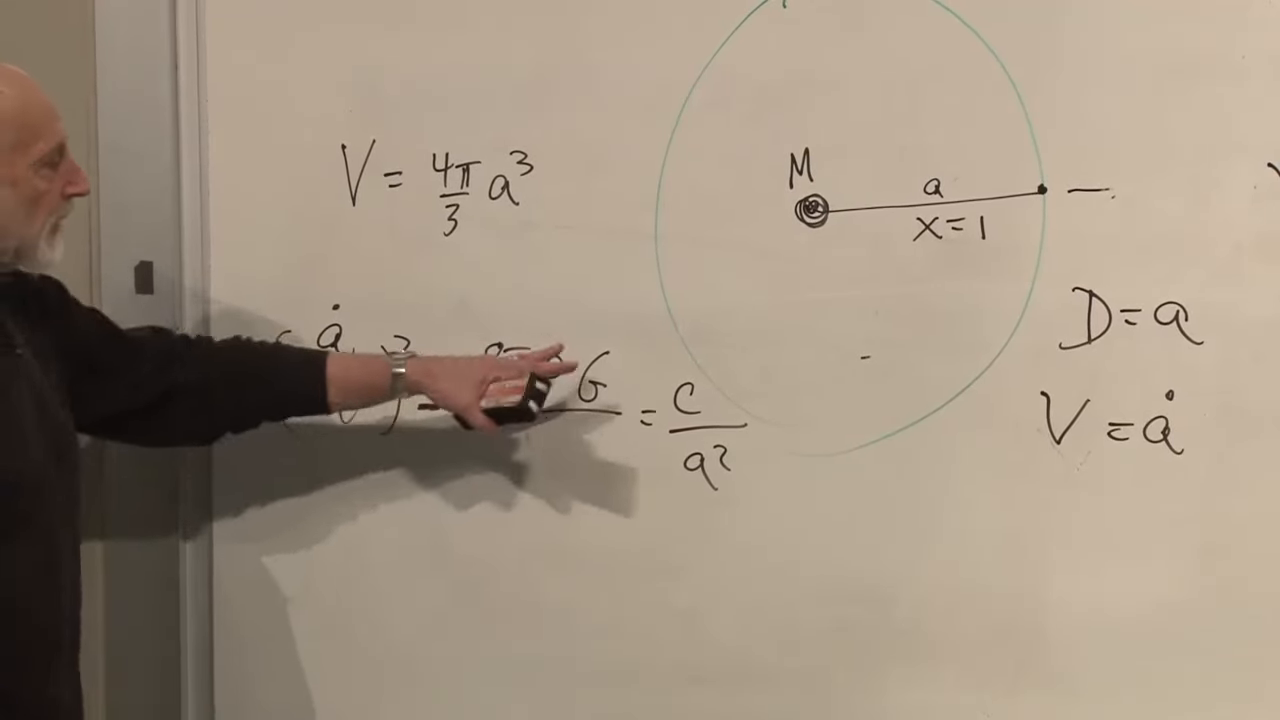
\includegraphics[width=0.86\textwidth]{lecture_02_figure_03.png}
\caption{La esfera de masa encerrada y la ecuación de Friedmann para energía distinta de cero. Las etiquetas visibles incluyen \(V_{\rm sph}=4\pi a^3/3\), la masa central \(M\), \(x=1\), \(D=a\) y \(\dot D=\dot a\). El profesor oculta parte de la ecuación; más abajo se reconstruye algebraicamente.}
\label{fig:c02-energy-board}
\lectureframe{00:37:59.876}
\end{figure}

\begin{figure}[ht]
\centering
\begin{tikzpicture}[scale=1.05,>=Latex]
  \draw[thick] (0,0) circle (2.6);
  \fill (0,0) circle (2.2pt) node[below left=2pt] {\(M(a)\)};
  \draw[thick,->] (0,0) -- (2.58,0);
  \fill (2.6,0) circle (2.2pt) node[right=4pt] {galaxy \(m\)};
  \node[above] at (1.30,0.04) {\(D=ax\)};
  \node[below] at (1.30,-0.04) {\(x=1\Rightarrow D=a\)};
  \draw[->,blue!60!black,thick] (2.63,0.18) -- (3.55,0.72)
    node[right] {\(\dot D=\dot a\)};
  \node at (0,-3.05) {\(M(a)=\frac{4\pi}{3}\rho_m a^3\)};
\end{tikzpicture}
\caption{Reconstrucción limpia de la esfera newtoniana en \(x=1\). Las capas exteriores se cancelan, por lo que la galaxia del borde solo responde a la masa encerrada.}
\label{fig:c02-sphere-redraw}
\end{figure}

Sustituyamos \(D=a\) en la ecuación~\eqref{eq:c02-newton-energy}, dividamos por \(m/2\) y definamos la constante
\begin{equation}
C\equiv\frac{2E}{m}.
\end{equation}
Obtenemos
\begin{equation}
\dot a^{\,2}-\frac{2GM(a)}{a}=C.
\label{eq:c02-energy-a}
\end{equation}
Al dividir por \(a^2\) y usar la ecuación~\eqref{eq:c02-enclosed-mass} se obtiene
\begin{equation}
\left(\frac{\dot a}{a}\right)^2-
\frac{8\pi G}{3}\rho_m=\frac{C}{a^2},
\label{eq:c02-energy-form}
\end{equation}
o, de forma equivalente,
\begin{equation}
\boxed{H^2=\frac{8\pi G}{3}\rho_m+\frac{C}{a^2}.}
\label{eq:c02-friedmann-C}
\end{equation}
Esta es la primera ecuación de Friedmann para materia sin presión, expresada según la convención newtoniana de energía. El nuevo término \(a^{-2}\) refleja si la galaxia representativa se puso en movimiento por encima, justo en o por debajo de la energía de escape.

Al sustituir \(\rho_m=\nu_m/a^3\), conviene definir
\begin{equation}
A_m\equiv\frac{8\pi G\nu_m}{3}>0,
\end{equation}
de modo que
\begin{equation}
H^2=\frac{A_m}{a^3}+\frac{C}{a^2},
\qquad
\dot a^{\,2}=\frac{A_m}{a}+C.
\label{eq:c02-energy-branches}
\end{equation}
La ecuación resulta más informativa si se examinan sus límites antes de integrarla directamente.

\subsection{Energía positiva}

Si \(C>0\), el término de materia \(A_m/a^3\) domina para valores pequeños de \(a\). Por tanto, la expansión temprana sigue la ley de la materia \(a\propto t^{2/3}\). Sin embargo, para valores grandes de \(a\), el término \(C/a^2\) domina en \(H^2\), o, de forma equivalente,
\begin{equation}
\dot a^{\,2}\longrightarrow C.
\end{equation}
La expansión se aproxima a una velocidad constante,
\begin{equation}
a(t)\sim\sqrt C\,t.
\label{eq:c02-positive-late}
\end{equation}
Este es el análogo cosmológico de lanzar una manzana a una velocidad superior a la de escape. La gravedad reduce continuamente su velocidad, pero, muy lejos, la manzana conserva una velocidad asintótica distinta de cero.

\subsection{Energía nula}

Para \(C=0\), la ecuación~\eqref{eq:c02-energy-branches} recupera la solución crítica \(a\propto t^{2/3}\). La expansión continúa sin límite mientras \(\dot a\) tiende a cero. Es el caso exacto de energía de escape.

\subsection{Energía negativa}

Si \(C=-|C|<0\), entonces
\begin{equation}
H^2=\frac{A_m}{a^3}-\frac{|C|}{a^2}
=\frac{A_m-|C|a}{a^3}.
\label{eq:c02-negative-energy}
\end{equation}
El factor de escala no puede superar
\begin{equation}
a_{\max}=\frac{A_m}{|C|},
\label{eq:c02-amax}
\end{equation}
porque allí el lado derecho se anula. La rama expansiva llega a \(a_{\max}\) con \(\dot a=0\); la continuación es la rama contractiva. En el cuadro newtoniano, esto corresponde a lanzar una manzana por debajo de la velocidad de escape: sube, se detiene y cae.

\begin{classroomqa}
\audiencequestion{¿Cómo puede el modelo volver a colapsar si el lado derecho es igual a \(H^2\) y, por tanto, no puede ser negativo?}
\lecturerresponse{Nunca se vuelve negativo. Durante la expansión, el lado derecho disminuye hasta anularse en \(a_{\max}\). Allí, \(H=0\). La solución pasa entonces de la raíz cuadrada positiva a la negativa y recorre de nuevo la región permitida con \(\dot a<0\). Una continuación tentadora, pero incorrecta, dejaría que la expresión atravesara el cero. No puede hacerlo: el cero es el límite, no un valor que pueda atravesar un \(H\) real. \lecturetimestamp{00:48:43--00:53:03}}
\end{classroomqa}

Así pues, las tres energías newtonianas dan lugar a tres historias cualitativamente distintas: recollapse para \(C<0\), escape crítico para \(C=0\) y expansión eterna con \(\dot a\) asintóticamente constante para \(C>0\). El sorprendente paso siguiente es que la relatividad general asigna a estos mismos casos un significado geométrico.

\section{De la energía a la curvatura}

Pasemos el término de energía de la ecuación~\eqref{eq:c02-friedmann-C} al lado geométrico y definamos
\begin{equation}
k\equiv-C.
\label{eq:c02-k-definition}
\end{equation}
Entonces,
\begin{equation}
\boxed{H^2+\frac{k}{a^2}=\frac{8\pi G}{3}\rho.}
\label{eq:c02-friedmann-k}
\end{equation}
En la pizarra se alterna entre \(C\), \(K\) y \(\kappa\), y al pasar el término al otro lado de la igualdad se incorpora un signo. La ecuación~\eqref{eq:c02-k-definition} fija nuestra convención: la energía newtoniana positiva corresponde a \(k<0\), la energía nula a \(k=0\) y la energía newtoniana negativa a \(k>0\).

\begin{figure}[ht]
\centering
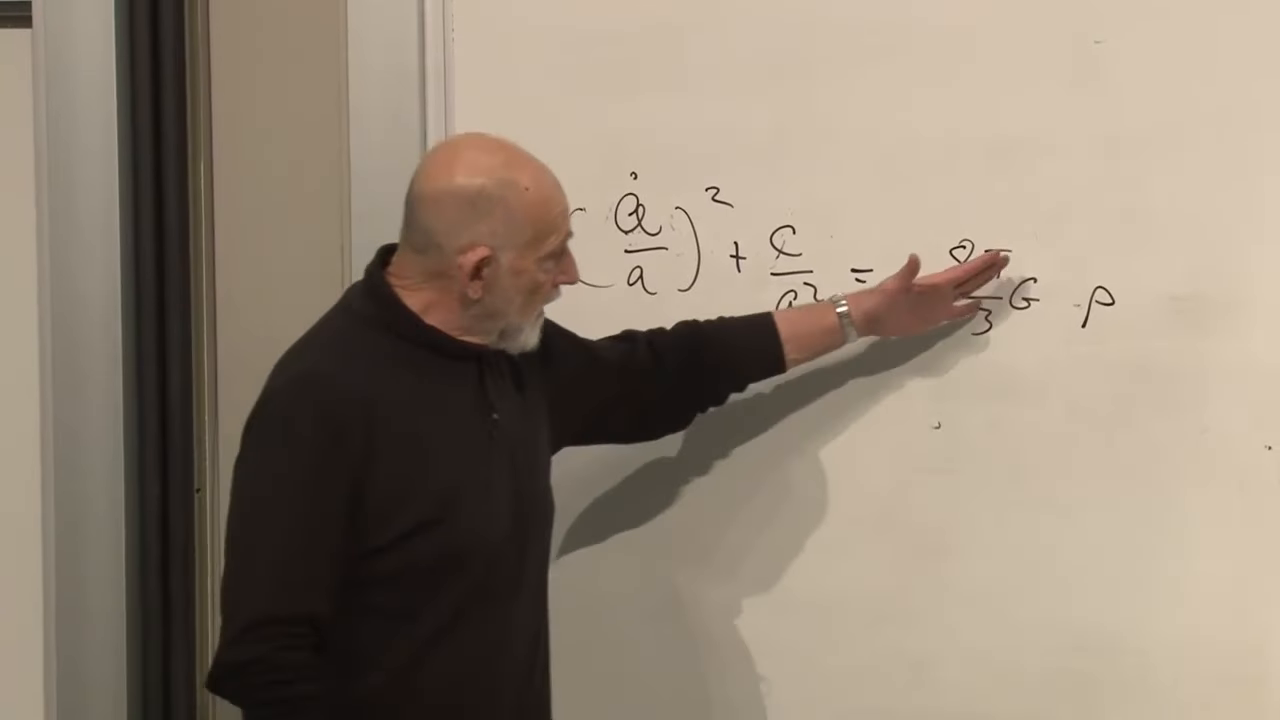
\includegraphics[width=0.76\textwidth]{lecture_02_figure_04.png}
\caption{La ecuación de Friedmann dispuesta con la geometría a la izquierda y la fuente a la derecha. El fotograma ilustra esta división conceptual; no muestra la ecuación tensorial completa de Einstein.}
\label{fig:c02-geometry-source}
\lectureframe{00:55:22.810}
\end{figure}

Esta disposición es una versión en miniatura de la ecuación de Einstein. El lado izquierdo describe la geometría: la expansión mediante \(H\) y la curvatura espacial mediante \(k/a^2\). El lado derecho describe la fuente material. En mecánica newtoniana, esa fuente era la densidad de masa. En relatividad es la energía y el momento, representados en su totalidad por el tensor de energía-momento. Para un universo homogéneo e isótropo, la primera ecuación de Friedmann depende de la densidad total de energía \(\rho\).

Si se mantienen las unidades ordinarias, una densidad de masa contribuye mediante su energía en reposo \(\rho_{\rm mass}c^2\). A partir de aquí adoptamos \(c=1\), de modo que masa y energía se expresan en las mismas unidades. El símbolo \(\rho\) puede incluir entonces la masa en reposo, la energía cinética, la radiación y cualquier otro componente homogéneo de energía.

\begin{figure}[ht]
\centering
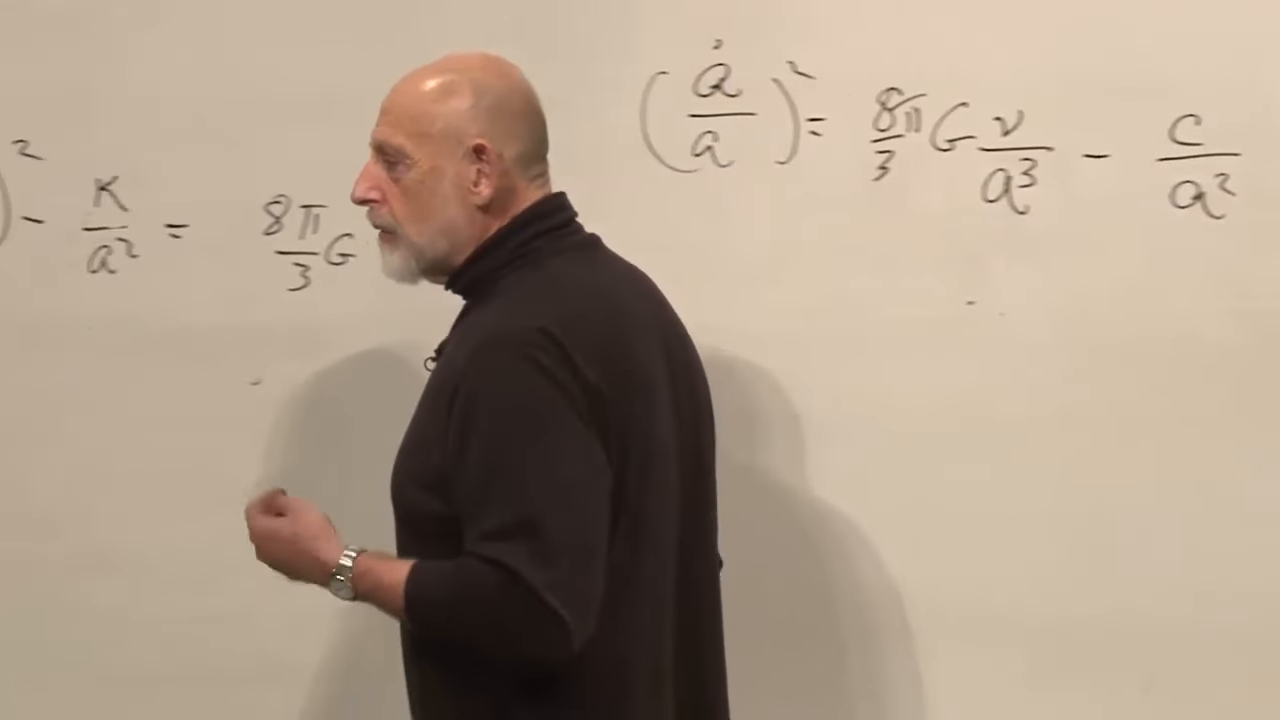
\includegraphics[width=0.88\textwidth]{lecture_02_figure_05.png}
\caption{Formas de la ecuación de Friedmann en la pizarra, una junto a otra: la forma con curvatura, que usa \(\rho\), y la forma con materia, obtenida tras sustituir \(\rho_m=\nu_m/a^3\). La notación de la pizarra cambia; la ecuación~\eqref{eq:c02-k-definition} mantiene fija aquí la convención de signos.}
\label{fig:c02-curvature-comparison}
\lectureframe{00:57:52.659}
\end{figure}

La interpretación geométrica es global. En el modelo relativista, \(k=0\) describe hipersuperficies espaciales planas; \(k>0\), hipersuperficies esféricas de curvatura positiva; y \(k<0\), hipersuperficies hiperbólicas de curvatura negativa. La derivación newtoniana reprodujo la misma ecuación de evolución sin contar con esas geometrías globales. Por tanto, su constante de energía distinta de cero imita la curvatura con notable precisión, pero no constituye una derivación del espacio curvo en sí.

\begin{classroomqa}
\audiencequestion{¿Cómo pueden la mecánica newtoniana y la relatividad general dar la misma ecuación de expansión si sus geometrías son distintas?}
\lecturerresponse{La relatividad general incluye el caso plano y, localmente, toda geometría suave es aproximadamente plana. Aún más notable es que la constante de energía newtoniana aparece en la ecuación de evolución exactamente en el lugar que ocupa la curvatura espacial relativista. La fórmula dinámica coincide, pero la interpretación global no: el espacio euclídeo newtoniano no se ha convertido secretamente en una esfera ni en un espacio hiperbólico. Las tres geometrías han de construirse dentro de la relatividad general. \lecturetimestamp{01:20:59--01:24:20}}
\end{classroomqa}

\section{La radiación en una caja en expansión}

Ahora cambiaremos el contenido del universo. Consideremos un cubo comóvil unitario. Su volumen físico es \(a^3\). En el caso de materia no relativista, el número de partículas de la caja es fijo y la energía en reposo de cada partícula se mantiene aproximadamente constante, lo que da \(\rho_m\propto a^{-3}\). En la radiación ocurre algo más: cada fotón pierde energía a medida que el universo se expande.

Un fotón de longitud de onda \(\lambda\) tiene una energía
\begin{equation}
E_\gamma=\frac{hc}{\lambda},
\qquad
E_\gamma\propto\lambda^{-1}.
\label{eq:c02-photon-energy}
\end{equation}
En una expansión homogénea, la longitud de onda de una onda que se propaga libremente se estira con el factor de escala:
\begin{equation}
\frac{\lambda(t_2)}{\lambda(t_1)}
=\frac{a(t_2)}{a(t_1)},
\qquad
\lambda\propto a.
\label{eq:c02-redshift}
\end{equation}
Esto es el corrimiento cosmológico al rojo. De ello se deduce que
\begin{equation}
E_\gamma\propto a^{-1}.
\label{eq:c02-photon-redshift}
\end{equation}
Si se conserva el número de fotones en la caja comóvil, su energía total de radiación disminuye como \(a^{-1}\). Al dividirla por su volumen físico \(a^3\), se obtiene
\begin{equation}
\boxed{\rho_r(a)=\frac{\nu_r}{a^4}.}
\label{eq:c02-radiation-density}
\end{equation}
Aquí \(\nu_r\) es la amplitud constante de la densidad de radiación que se propaga libremente. La radiación tiene una potencia inversa adicional de \(a\) respecto de la materia: tres potencias debidas a la dilución espacial y una al corrimiento al rojo de cada fotón.

La analogía de la cuerda de guitarra ofrece una intuición útil. Un modo que se ajusta a una cuerda tiene un número entero de semilongitudes de onda. Si la cuerda se alarga lentamente, ese entero no puede cambiar de forma continua; en cambio, la longitud de onda se ajusta a la nueva longitud. Del mismo modo, para una onda en un anillo que se expande lentamente, el número de nodos es un invariante adiabático, así que su longitud de onda sigue la circunferencia. Una onda general puede descomponerse en esos modos.

Esto no sustituye la resolución de las ecuaciones de Maxwell en un espacio-tiempo en expansión. Es la intuición controlada que subyace a la ecuación~\eqref{eq:c02-redshift}: una expansión geométrica lenta cambia la longitud de onda física y conserva la etiqueta del modo.

\begin{classroomqa}
\audiencequestion{¿Este argumento requiere una caja conductora o reflectante? ¿Qué ocurre en un espacio vacío en expansión, sin paredes físicas?}
\lecturerresponse{Las paredes son un recurso contable, no una afirmación de que el universo esté encerrado por un conductor. Una demostración completa se obtiene a partir de la propagación de ondas en la métrica en expansión. Para el argumento actual usamos el hecho observado y derivado relativísticamente de que las longitudes de onda que se propagan libremente escalan con \(a\). La caja ayuda a contar los fotones y el volumen físico; no causa el corrimiento cosmológico al rojo. \lecturetimestamp{01:02:21--01:04:37}}
\end{classroomqa}

\begin{classroomqa}
\audiencequestion{¿Por qué habría de seguir una longitud de onda a la cuadrícula en vez de mantener una longitud física fija?}
\lecturerresponse{Consideremos un modo en un anillo cuya circunferencia cambia adiabáticamente. Su número entero de nodos no puede variar de forma continua, así que la longitud de onda permitida debe cambiar con el anillo. Si se descompone una onda general en modos de Fourier, se llega a la misma conclusión para cada modo. Esto aporta la intuición adiabática necesaria; el enunciado exacto corresponde a la teoría de campos en el espacio-tiempo curvo. \lecturetimestamp{01:34:18--01:38:33}}
\end{classroomqa}

\subsection{La solución dominada por la radiación}

Por el momento, omitamos la curvatura e insertemos la ecuación~\eqref{eq:c02-radiation-density} en la ecuación de Friedmann:
\begin{equation}
H^2=\frac{8\pi G\nu_r}{3a^4}
\equiv\frac{A_r}{a^4},
\qquad A_r>0.
\label{eq:c02-radiation-friedmann}
\end{equation}
En la rama expansiva,
\begin{equation}
\frac{\dot a}{a}=\frac{\sqrt{A_r}}{a^2},
\qquad
\dot a=\frac{\sqrt{A_r}}{a}.
\end{equation}
Por tanto,
\begin{equation}
a\,da=\sqrt{A_r}\,dt,
\qquad
\frac{a^2}{2}=\sqrt{A_r}(t-t_B),
\end{equation}
y
\begin{equation}
\boxed{a(t)\propto(t-t_B)^{1/2}.}
\label{eq:c02-radiation-law}
\end{equation}
La diferencia entre los exponentes \(1/2\) y \(2/3\) parece pequeña a la vista, pero es decisiva desde el punto de vista físico. La tasa de expansión, la temperatura, la congelación de las reacciones y el tamaño del horizonte en el universo temprano dependen de cuál componente domine.

\section{Un universo de materia y radiación}

Si la materia y la radiación se conservan por separado, sus densidades se suman:
\begin{equation}
\rho(a)=\rho_m(a)+\rho_r(a).
\end{equation}
Si se ignora la curvatura para esta comparación,
\begin{equation}
\boxed{H^2=\frac{C_m}{a^3}+\frac{C_r}{a^4},}
\label{eq:c02-mixed-friedmann}
\end{equation}
donde \(C_m,C_r>0\). En la pizarra se asignan primero a los dos coeficientes las etiquetas \(C_1\) y \(C\); verbalmente, el segundo símbolo se corrige para designar una constante distinta. La notación de la ecuación~\eqref{eq:c02-mixed-friedmann} deja explícita esa corrección.

\begin{figure}[ht]
\centering
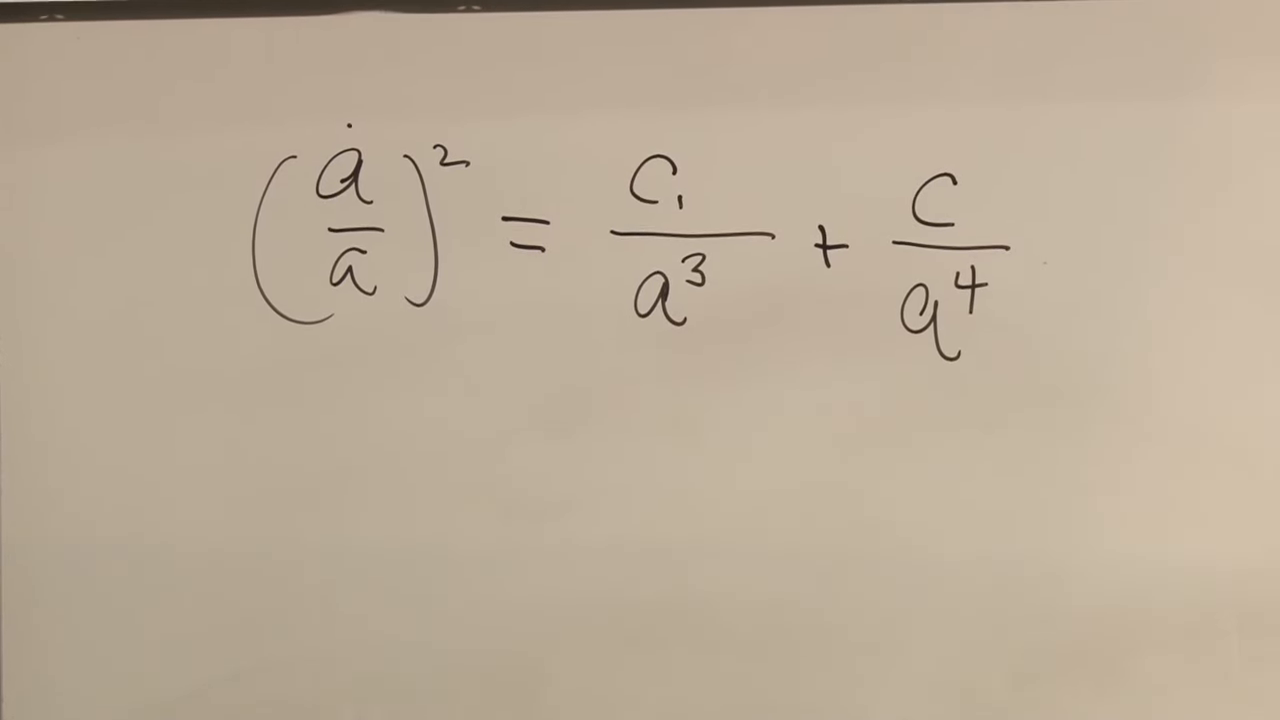
\includegraphics[width=0.74\textwidth]{lecture_02_figure_06.png}
\caption{La ecuación para la mezcla de materia y radiación escrita en la pizarra. Más adelante se corrige el segundo coeficiente escrito y se sustituye por una constante específica de la radiación, denotada por \(C_r\) en la ecuación~\eqref{eq:c02-mixed-friedmann}.}
\label{fig:c02-mixed-board}
\lectureframe{01:11:37.997}
\end{figure}

Para valores pequeños de \(a\), domina el término de radiación, porque \(a^{-4}\) crece más deprisa que \(a^{-3}\):
\begin{equation}
a\ll a_{\rm eq}
\quad\Longrightarrow\quad
H^2\simeq\frac{C_r}{a^4},
\qquad
a(t)\propto t^{1/2}.
\end{equation}
Para valores mayores de \(a\), domina la materia:
\begin{equation}
a\gg a_{\rm eq}
\quad\Longrightarrow\quad
H^2\simeq\frac{C_m}{a^3},
\qquad
a(t)\propto t^{2/3}.
\end{equation}
La escala de igualdad se obtiene directamente al igualar ambos términos:
\begin{equation}
a_{\rm eq}=\frac{C_r}{C_m}.
\label{eq:c02-equality-scale}
\end{equation}
Esta igualdad no coincide con el desacoplamiento de los fotones. La igualdad señala cuándo coinciden las dos densidades de energía; el desacoplamiento, cuándo las interacciones dejan de mantener la materia y la radiación en contacto térmico.

El sector de radiación incluye los fotones y cualquier especie que se mueva de forma ultrarrelativista. Los neutrinos muy ligeros se comportan así a temperaturas suficientemente altas, y un fondo de gravitones escalaría del mismo modo. Cuando una especie masiva se vuelve no relativista, su contribución dominante de masa en reposo empieza a escalar como la materia. La materia oscura fría pertenece a \(C_m/a^3\), no al término de radiación.

\begin{classroomqa}
\classquestion{¿Qué término de la ecuación~\eqref{eq:c02-mixed-friedmann} domina primero y cuál domina más tarde?}
\lecturerresponse{Para valores pequeños de \(a\), \(a^{-4}\) crece más deprisa que \(a^{-3}\), así que la radiación controla la expansión temprana y da \(a\propto t^{1/2}\). A medida que \(a\) crece, la razón entre radiación y materia disminuye como \(1/a\); entonces la materia controla la expansión y da \(a\propto t^{2/3}\). \lecturetimestamp{01:11:46--01:13:38}}
\end{classroomqa}

\begin{classroomqa}
\audiencequestion{¿Se supone que las cantidades relativas de materia y radiación permanecen constantes?}
\lecturerresponse{Sus densidades no son constantes, pero los coeficientes \(C_m\) y \(C_r\) pueden considerarse constantes una vez que los componentes dejan de intercambiar energía de forma eficiente y la creación o aniquilación de partículas se vuelve despreciable. Entonces la materia conserva una masa en reposo comóvil y la radiación libre, un número comóvil de fotones; el corrimiento al rojo aporta el factor adicional \(a^{-1}\). Durante épocas de interacciones intensas o aniquilación de especies, hay que refinar la contabilidad. \lecturetimestamp{01:13:39--01:14:53}}
\end{classroomqa}

\begin{classroomqa}
\audiencequestion{¿Cuándo dejaron de interactuar intensamente la materia y la radiación?}
\lecturerresponse{Una respuesta aproximada, en orden de magnitud, es \(10^5\) años para el desacoplamiento de los fotones respecto de la materia ordinaria. La historia precisa de la recombinación se calcula más adelante y no debe confundirse con la igualdad entre materia--radiación. Aquí solo necesitamos que, después del desacoplamiento, los dos componentes puedan seguirse aproximadamente por separado. \lecturetimestamp{01:27:29--01:27:46}}
\end{classroomqa}

\begin{classroomqa}
\audiencequestion{¿Cómo sabemos que hubo una era temprana con \(a\propto t^{1/2}\) antes de que existieran galaxias que permitieran seguir la expansión?}
\lecturerresponse{Inferimos la historia de la expansión a partir de los registros físicos que deja. La nucleosíntesis primordial depende de la competencia temprana entre las tasas de reacción y \(H(t)\); el fondo cósmico de microondas registra el estado térmico posterior y las perturbaciones. Las observaciones de galaxias permiten constatar de manera más directa el comportamiento de la era dominada por la materia, mientras que la era de radiación se reconstruye a partir de estas pruebas del universo temprano. \lecturetimestamp{01:27:46--01:30:10}}
\end{classroomqa}

El modelo de materia más radiación es deliberadamente incompleto. Se trata del marco clásico en el que el universo pasa de estar dominado por la radiación a estar dominado por la materia. La expansión acelerada actual requiere otra fuente, la energía oscura, que añadirá un término de carácter cualitativamente distinto.

\section{Adónde va la energía desplazada al rojo}

La disminución \(E_\gamma\propto a^{-1}\) plantea una pregunta inevitable: ¿adónde ha ido la energía de los fotones? En una caja literal en expansión con paredes reflectantes, la radiación ejerce presión y realiza trabajo sobre las paredes. La expresión termodinámica es
\begin{equation}
dE=-p\,dV.
\label{eq:c02-pdv}
\end{equation}
Al aumentar \(V\), disminuye la energía de la radiación. La energía perdida puede aparecer como energía cinética, deformación o calor en aquello que mueva las paredes.

La caja comóvil no tiene paredes materiales. Es un límite imaginario que se mueve con la expansión media. Los fotones lo atraviesan, pero, en un baño de radiación homogéneo, el flujo estadístico que entra compensa el que sale. La caja sigue siendo un volumen contable válido aunque no sea un recipiente. La ley del trabajo de presión sigue describiendo cómo evoluciona la energía en un volumen comóvil.

Para la radiación, \(p=\rho/3\), y \(E=\rho V\). La ecuación~\eqref{eq:c02-pdv} da entonces
\begin{align}
d(\rho V)&=-\frac{\rho}{3}\,dV,\\
V\,d\rho&=-\frac{4}{3}\rho\,dV,\\
\frac{d\rho}{\rho}&=-\frac{4}{3}\frac{dV}{V}.
\end{align}
Como \(V\propto a^3\), la integración da \(\rho\propto a^{-4}\), en concordancia con el argumento basado en la longitud de onda. Esta derivación termodinámica también deja claro que disminuye la energía de cada fotón, y no solo la densidad numérica.

\begin{classroomqa}
\audiencequestion{¿Adónde va la energía de los fotones desplazados al rojo? ¿Se conserva la energía total del cosmos?}
\lecturerresponse{Si hay paredes físicas, la radiación realiza trabajo sobre ellas y la transferencia se describe mediante la contabilidad mecánica ordinaria. Para el universo en su conjunto, la cuestión es más sutil. La conservación global de la energía suele derivarse de la simetría ante traslaciones temporales, pero un espacio-tiempo en expansión no suele ser invariante ante traslaciones temporales y puede no tener una energía total conservada única. Se pueden construir analogías newtonianas útiles en las que interviene la energía de expansión, pero para una afirmación global definitiva se requiere la relatividad general. Ambas descripciones son útiles aquí, pero el modelo newtoniano no permite llegar a una conclusión global definitiva. \lecturetimestamp{01:16:51--01:20:58}}
\end{classroomqa}

\begin{classroomqa}
\audiencequestion{Si la caja comóvil es imaginaria y los fotones atraviesan sus límites, ¿cómo puede seguir siendo útil la imagen del trabajo de presión?}
\lecturerresponse{La homogeneidad proporciona la contabilidad que falta. En promedio, cada fotón que sale de un volumen comóvil es sustituido estadísticamente por uno que entra desde el volumen vecino. Los flujos locales se cancelan en promedio, mientras cambian el volumen físico y las longitudes de onda. Una caja reflectante hace concreto el mecanismo del trabajo; la caja comóvil expresa la misma ley de conservación promediada sin paredes literales. \lecturetimestamp{01:24:22--01:27:28}}
\end{classroomqa}

\begin{classroomqa}
\audiencequestion{¿La expansión solo reduce la densidad de fotones o también reduce la energía de cada fotón?}
\lecturerresponse{Ocurren ambas cosas. El número de fotones por volumen físico disminuye como \(a^{-3}\) y el corrimiento cosmológico al rojo reduce la energía de cada fotón en un factor adicional \(a^{-1}\). Es el análogo radiativo del enfriamiento adiabático. Un gas ordinario también se enfría mientras realiza trabajo durante una expansión lenta, aunque una expansión libre repentina es un proceso termodinámico distinto. \lecturetimestamp{01:42:30--01:45:55}}
\end{classroomqa}

\section{Recesión, horizontes y límites del modelo}

La ley de Hubble asigna una velocidad de recesión
\begin{equation}
v_{\rm rec}=HD
\label{eq:c02-recession}
\end{equation}
a un objeto situado a una distancia propia \(D\) en una hipersuperficie de tiempo cósmico elegida. Para valores suficientemente grandes de \(D\), la ecuación~\eqref{eq:c02-recession} puede superar \(c\). Esto no viola la relatividad especial, porque \(v_{\rm rec}\) no es la velocidad de un objeto cercano medida en un único sistema inercial local. Compara líneas de universo comóviles muy separadas dentro de una geometría cambiante. Todo observador local sigue midiendo la velocidad de la luz como \(c\), y ningún objeto material local adelanta a otro a una velocidad superior a la de la luz.

\begin{classroomqa}
\audiencequestion{¿Puede una galaxia suficientemente distante alejarse más rápido que la luz?}
\lecturerresponse{Sí, su tasa de recesión cosmológica \(HD\) puede superar \(c\). Ningún objeto local adelanta entonces a un observador vecino más rápido que la luz, y este resultado no puede utilizarse para transmitir señales superlumínicas. Se trata de una afirmación sobre el cambio de la distancia propia entre líneas de universo comóviles distantes, no de una velocidad ordinaria de la relatividad especial medida en un único suceso. \lecturetimestamp{01:30:17--01:32:13}}
\end{classroomqa}

La recesión superlumínica, por sí sola, no determina si la luz emitida ahora llegará alguna vez hasta nosotros. Esa cuestión depende de toda la historia futura de la expansión. En un modelo desacelerado dominado por la materia, regiones que actualmente se alejan más rápido que la luz pueden volverse observables más adelante, porque el horizonte pertinente evoluciona. Si persiste la expansión acelerada, un horizonte de sucesos puede ocultar para siempre los sucesos suficientemente distantes.

\begin{classroomqa}
\audiencequestion{¿Desaparecen las galaxias cuando su tasa de recesión supera la velocidad de la luz?}
\lecturerresponse{No necesariamente. El cruce del radio de Hubble y un verdadero horizonte de sucesos son conceptos distintos. En un modelo desacelerado, la luz procedente de una región que actualmente se aleja a una velocidad superlumínica aún puede alcanzarnos más adelante. La dominación persistente de la energía oscura cambia la estructura causal global y puede crear un horizonte definitivo. Para determinar qué señales llegan se necesita la geometría del espacio-tiempo, no una instantánea de \(HD\). \lecturetimestamp{01:32:14--01:34:18}}
\end{classroomqa}

El lenguaje de la relatividad especial también puede inducir a error cuando se aplica globalmente. La masa en reposo invariante de una partícula no aumenta con la velocidad. Su energía y su momento dependen del sistema de referencia local del observador. Las partículas masivas no pueden acelerarse hasta superar la velocidad local de la luz, pero la recesión de una galaxia comóvil distante no equivale a su paso por un único sistema de referencia local.

\begin{classroomqa}
\audiencequestion{¿Adquiere una galaxia que se aleja rápidamente una masa relativista mayor?}
\lecturerresponse{Es más claro evitar el término ``masa relativista.'' La galaxia tiene una masa en reposo invariante, mientras que su energía y su momento dependen del sistema de referencia. Además, una tasa de recesión asignada a través de una distancia cosmológica no es la velocidad local que aparece en la fórmula de la relatividad especial. Estos conceptos concuerdan solo cuando se comparan los sucesos distantes mediante la métrica del espacio-tiempo. \lecturetimestamp{01:38:34--01:40:05}}
\end{classroomqa}

\begin{classroomqa}
\audiencequestion{¿Qué ocurre con los ejes del tiempo y del espacio cuando una tasa de recesión distante es superlumínica?}
\lecturerresponse{No existe un único sistema de Lorentz global cuyos ejes inclinados resuelvan la cuestión. La relatividad especial compara sistemas inerciales en un espacio-tiempo plano; la cosmología requiere una métrica que relacione sistemas locales a lo largo de un espacio-tiempo curvo extendido. El razonamiento newtoniano sigue siendo fiable en una región pequeña, pero para la construcción global hay que esperar a la relatividad general. \lecturetimestamp{01:40:07--01:42:30}}
\end{classroomqa}

La conservación de la energía newtoniana ha dado la ecuación correcta del factor de escala para la materia e incluso ha anticipado el término de curvatura. La mecánica ondulatoria y la termodinámica proporcionan la ley de escala de la radiación. Sin embargo, la geometría espacial, la energía global y los horizontes no son cuestiones newtonianas locales: requieren la descripción métrica que viene a continuación.

\section{Materia, radiación y curvatura}

La solución crítica con solo materia satisface
\begin{equation}
\rho_m\propto a^{-3},
\qquad
a(t)\propto t^{2/3}.
\end{equation}
Al restituir la energía newtoniana por unidad de masa, se obtiene
\begin{equation}
H^2=\frac{8\pi G}{3}\rho_m+\frac{C}{a^2}.
\end{equation}
Un valor positivo de \(C\) da lugar a una expansión eterna, con \(a\sim t\) en tiempos tardíos; \(C=0\) corresponde al escape crítico, y un valor negativo de \(C\) produce un factor de escala máximo seguido de un recolapso. Al definir \(k=-C\), el mismo término queda en el lado geométrico de la ecuación relativista de Friedmann.

La radiación se diferencia de la materia porque la expansión modifica tanto la densidad numérica como la energía de cada cuanto:
\begin{equation}
\begin{aligned}
\lambda&\propto a,
&\qquad E_\gamma&\propto a^{-1},\\
\rho_r&\propto a^{-4},
& a(t)&\propto t^{1/2}.
\end{aligned}
\end{equation}
Por tanto, la ecuación de dos componentes
\begin{equation}
H^2=\frac{C_m}{a^3}+\frac{C_r}{a^4}
\end{equation}
describe un universo temprano dominado por la radiación, seguido de una era dominada por la materia. La energía oscura, la geometría espacial y la estructura causal de los horizontes quedan fuera de este modelo; es precisamente en ese punto donde la aproximación newtoniana nos indica que debemos dejar el problema en manos de la relatividad general.
